\begin{frame}{Hetergeneous Multiscale Molecular Dynamics (HMMD)}
\begin{tikzpicture}[scaleall=1.0]
\pcuad{\textwidth}{\textheight}
\path(nw) ++(0,0) node(graphic1)[anchor=north west]{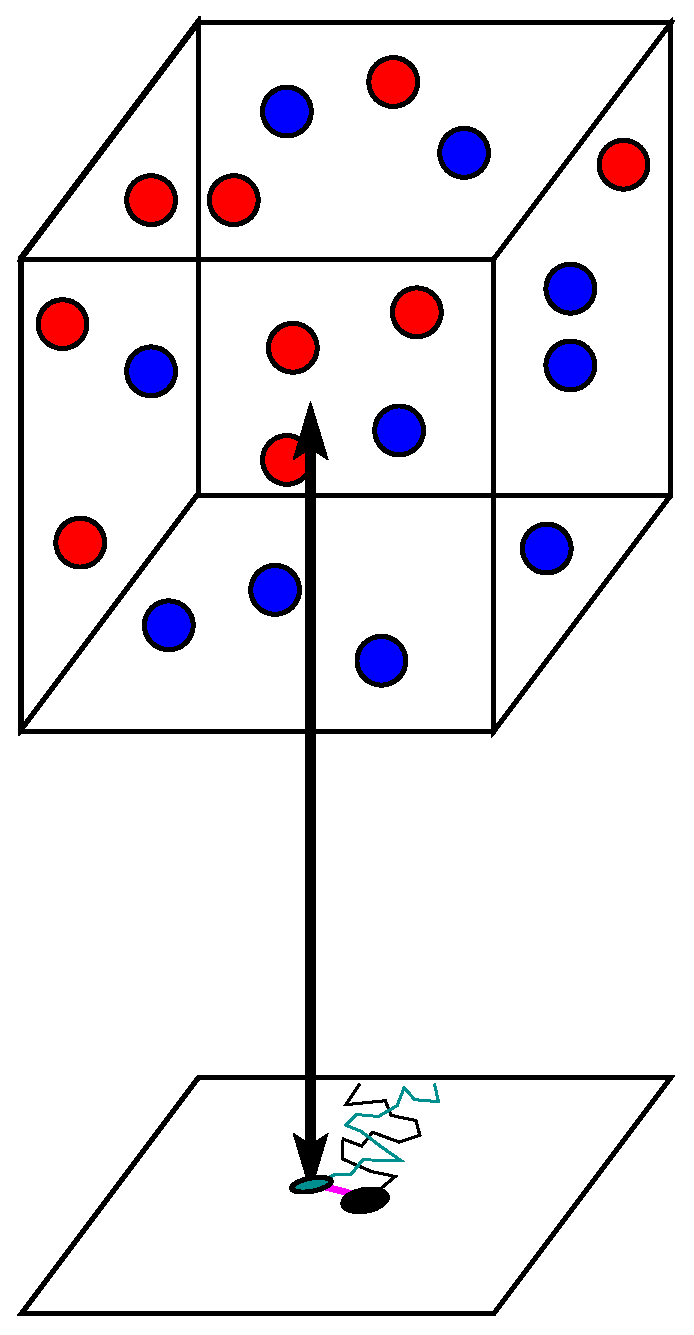
\includegraphics[width=0.35\textwidth]{hmmd-graphic2.eps}};
\path(graphic1) ++(2,3) node(label1)[anchor=north west, text width=0.7\textwidth]{$\displaystyle m_i\ddot{x}_i = -\nabla_iV(\xb)-\sum_{j=1}^M\kappa[\theta_j(\xb)-z_j]\frac{\partial\theta_j}{\partial x_i} + \mbox{e.f.}$};
\path(graphic1) ++(2,-2) node(label3)[anchor=north west, text width=0.7\textwidth]{$\displaystyle\bar{m}_j\ddot{z}_j = \sum_{k=1}^{M} \mathcal{M}_{jk}\kappa[\theta_k(\xb)-z_k] + \mbox{e.f.}$};
\draw[magenta,thick,rounded corners] (6,5) rectangle (9,6);
\draw[magenta,thick] (7.5,5.5) node[align=left] {Forces link $\xb$ and $\zb$};
\draw[thick,rounded corners] (5,3.5) rectangle (10,4.5);
\draw[thick] (7.5,4) node[align=left] {Bias on $\zb$: Enhanced sampling\\of feature space};
\draw[] (1.25,2) node {$\thetab(\xb)$};
\draw[] (2.5,1.75) node {$\zb$};
\end{tikzpicture}
\end{frame}
